\section{Transaktionsinterface}
Anwendungen interagieren über das \acrshort{dbms} mit der \acrshort{db}. Damit die Grenzen der Transaktion eindeutig sind, signalisiert die Anwendung den Beginn einer Transaktion (\textit{Begin}). Nach der Ausführung der gewünschten Operationen muss dem \acrshort{dbms} der erfolgreiche oder erfolglose Abschluss (\textit{Commit} oder \textit{Rollback}) signalisiert werden\cite{Dey.}. Das \acrshort{dbms} bietet dem Entwickler der Anwendung diese drei Kommandos an.

\section{Verteilte Transaktionen}
In verteilten Systemen kann die Anforderung bestehen, dass eine Aktion mehrere Datenquellen verändern muss. Von dieser Aktion wird oft erwartet, dass sie ACID-Eigenschaften gewährleistet. Besonders die Atomarität einer solchen Transaktion stellt eine große Herausforderung in verteilten Systemen dar. 

Die Komplexität verteilter Transaktionen entsteht vordergründig durch das potentielle Auftreten von Netzwerkfehlern. Ist ein Transaktionsteilnehmer vorübergehend nicht erreichbar, ist der Zustand der \acrshort{llt} ungewiss. Es ist nicht eindeutig, ob die im nicht erreichbaren Teilnehmer stattfindende Operation ausgeführt wurde oder nicht. Deshalb ist auch die Entscheidung spekulativ, ob die erfolgreich absolvierten Teiloperationen zurückgerollt werden müssen oder nicht. In jedem Bereich der verteilten Transaktion können Netzwerkfehler auftreten. 

Systemabstürze stellen ebenfalls eine Herausforderung für verteilte Transaktionen dar. Es ist unklar, ob ein Teilnehmerservice abgestürzt ist bevor oder nachdem die Änderungen committet wurden. 

Als Lösung für diese Herausforderungen wurden Protokolle für verteilte Transaktionen entwickelt. 

\section{Zwei-Phasencommit}
Der \acrfull{2pc} ist ein solches Protokoll. Es besteht aus 2 Phasen: der \textit{Prepare}- und der \textit{Commit-Phase}. Die Transaktion wird von einem Koordinator gesteuert. 

\paragraph*{Prepare-Phase} \mbox{} \\
Der Koordinator signalisiert allen Transaktionsteilnehmer den Beginn der Transaktion. Die Transaktionsteilnehmer antworten entweder mit einem \textit{ready} oder \textit{failed}. Im Falle eines \textit{ready} muss der Transaktionsteilnehmer garantieren, dass er seine Operation fehlerfrei committen kann. Dabei werden die zu verändernden Ressourcen gesperrt. 

\paragraph*{Commit-Phase} \mbox{} \\
Der Koordinator wartet bis alle Teilnehmer geantwortet haben. Signalisieren alle Antworten einen Erfolg, fordert der Koordinator alle Teilnehmer zu einem Commit auf. Der Commit wird von allen Teilnehmern bestätigt.

Erhält der Koordinator in der \textit{Prepare-Phase} mindestens ein \textit{failed}, werden im Anschluss alle Teilnehmer zu einem Rollback aufgefordert. Auch diesen müssen wieder alle Teilnehmer bestätigen\cite{Gaitonde.24.03.2021}. 

\begin{figure}[!htbp]
	\begin{minipage}{.45\textwidth}
		\centering
		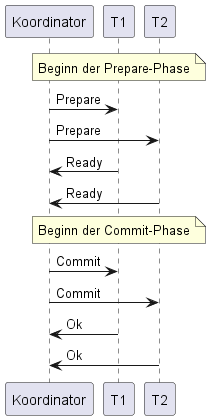
\includegraphics[height=8cm]{figures/ChapterGrundlagen/2pcSuccess-0.png}
		\caption{Sequenzdiagramm für erfolgreichen \acrshort{2pc}}
		\label{fig:2pcsucces}
	\end{minipage}
	\hfill
	\hfill
	\begin{minipage}{.45\textwidth}
		\centering
		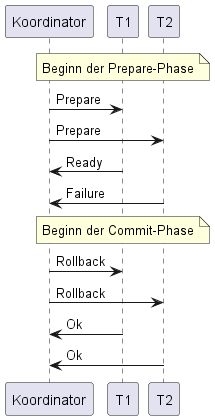
\includegraphics[height=8cm]{figures/ChapterGrundlagen/2pcFailure-0.png}
		\caption{Sequenzdiagramm für erfolglosen \acrshort{2pc}}
		\label{fig:2pcfailure}
	\end{minipage}
\end{figure}
\FloatBarrier

\paragraph*{Nachteile des \acrshort{2pc}} \mbox{} \\
\begin{itemize}
	\item \textbf{Blockierendes Verhalten}: Da in der \textit{Prepare-Phase} das Versprechen der Teilnehmer besteht, eine Transaktion committen zu können, müssen die zu verändernden Ressourcen gesperrt werden. Dies stellt sicher, dass die Transaktion von anderen Transaktionen isoliert ist. 
	\item \textbf{Blockierendes Verhalten bei Ausbleiben einer Antwort}: Treten Netzwerkfehler auf, dann bleiben die Locks so lange bestehen, bis die Netzwerkpartition wieder aufgelöst ist. Auch im \acrshort{2pc} hat der Koordinator keine Kenntnis über den Ausführungsstand im Teilnehmer falls eine Antwort ausbleibt.  
	\item \textbf{Starke Bindung}: Der Koordinator ist sehr eng mit den Teilnehmern gekoppelt.
	\item \textbf{Single Point of Failure}: Der Koordinator stellt eine kritische Komponente dar. Fällt der Koordinator aus, bleiben die Locks der Transaktionsteilnehmer bestehen.
\end{itemize}
